\documentclass{article}%
\usepackage[T1]{fontenc}%
\usepackage[utf8]{inputenc}%
\usepackage{lmodern}%
\usepackage{textcomp}%
\usepackage{lastpage}%
\usepackage[head=40pt,margin=0.5in,bottom=0.6in]{geometry}%
\usepackage{graphicx}%
%
\title{\textbf{Muere niño de 12 años por una bala perdida en la avenida Bolívar}}%
\author{Diario El Universal}%
\date{11/10/2018}%
%
\begin{document}%
\normalsize%
\maketitle%
\textbf{URL: }%
http://www.eluniversal.com/sucesos/22912/muere{-}nino{-}de{-}12{-}anos{-}por{-}una{-}bala{-}perdida{-}en{-}la{-}avenida{-}bolivar\newline%
%
\textbf{Periodico: }%
EU, %
ID: %
22912, %
Seccion: %
sucesos\newline%
%
\textbf{Palabras Claves: }%
NO\_TIENE\newline%
%
\textbf{Derecho: }%
1.1, %
Otros Derechos: %
, %
Sub Derechos: %
1.1.1.9\newline%
%
\textbf{EP: }%
NO\newline%
\newline%
%
\textbf{\textit{En horas de la mañana se registró un enfrentamiento entre delincuentes y funcionarios policiales en la avenida Bolívar de Caracas dejando como saldo un menor muerto}}%
\newline%
\newline%
%
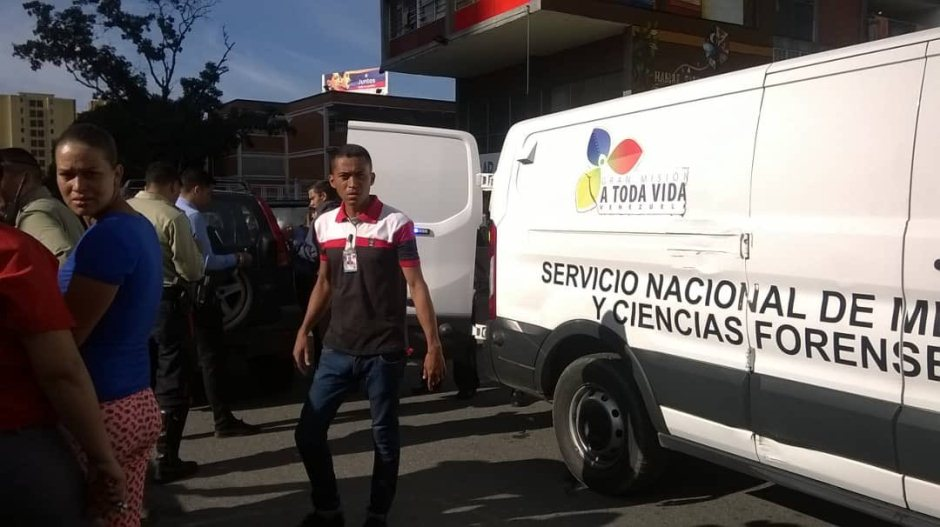
\includegraphics[width=300px]{162.jpg}%
\newline%
%
A primeras horas de la mañana se registró un enfrentamiento en la avenida Bolívar, de Caracas, donde resultó muerto un menor de 12 años por una bala perdida, según informa el periodista Roman Camacho, a través de su cuenta en Twitter%
\newline%
%
Destaca que el hecho ocurrió exactamente en el cruce de la Av Bolívar al frente al edificio de~ la Gran Misón Vivienda Venezuela, Oscar López Rivera, al lado del Museo de Los Niños.%
\newline%
%
Asimismo indica que según familiares, el niño vio a los antisociales cuando pasaban en el vehículo y le comenta al papá “ahí hay unos hombres con un revólver en la mano”, los sujetos se esconden, llega la PNB se escuchan los disparos del enfrentamiento.%
\newline%
%
\end{document}